\documentclass[tikz,border=3pt]{standalone}
\usetikzlibrary{positioning,arrows.meta,shapes.geometric,backgrounds}

\begin{document}
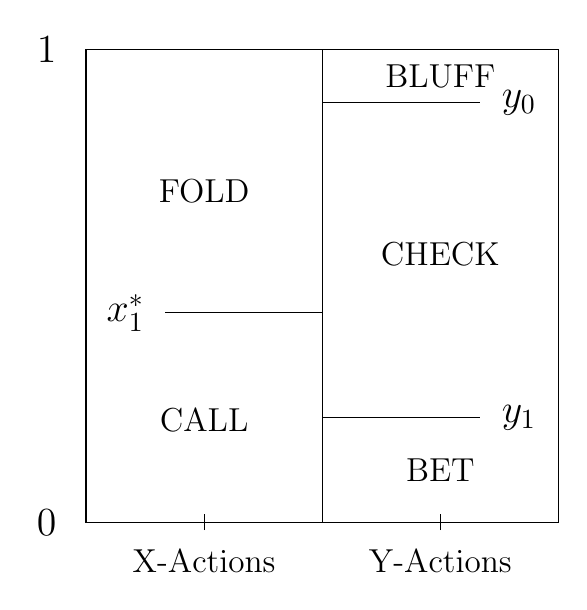
\begin{tikzpicture}

\draw (0,0) rectangle(6,6);
\draw (3,0) --(3,6);
\draw (3,1.33) --(5,1.33); %y1のライン
\draw (3,5.33) --(5,5.33); %y1のライン
\draw (3,2.66) --(1,2.66); %x1starのライン

\draw (1.5,-0.1) --(1.5,0.1);
\draw (4.5,-0.1) --(4.5,0.1);

\node[font=\Large] at (-0.5,0) {$0$};
\node[font=\Large] at (-0.5,6) {$1$};
\node[font=\large] at (1.5, -0.5) {X-Actions};
\node[font=\large] at (4.5, -0.5) {Y-Actions};
\node[font=\Large] at (5.5, 1.33) {$y_1$};
\node[font=\Large] at (5.5, 5.33) {$y_0$};
\node[font=\Large] at (0.5, 2.66) {$x_1^*$};

\node[font=\large] at (1.5, 4.2) {FOLD};
\node[font=\large] at (1.5, 1.3) {CALL};
\node[font=\large] at (4.5, 3.4) {CHECK};
\node[font=\large] at (4.5, 0.66) {BET};
\node[font=\large] at (4.5, 5.66) {BLUFF};

\end{tikzpicture}
\end{document}
